\documentclass{beamer}

\usetheme{Frankfurt}
\usecolortheme{dolphin}

\usepackage{amsmath, amssymb, amsfonts, tikz}
\usepackage[utf8]{inputenc}
\usepackage[T1]{fontenc}
\usepackage[english]{babel}

\DeclareTextFontCommand{\emph}{\bfseries}


\hypersetup{pdfstartview={Fit}}

\author{Alex J. Best}
\institute{WMS Talks}
\date{4/2/2014}
\title{Riemann Hypotheses}

\begin{document}

\section{Introduction}

\frame{\titlepage}

\begin{frame}
\frametitle{In this talk:}
\tableofcontents
\note{somebody (joshua if there) asked if I could prove the RH during this talk, and I am happy to announce that I will prove _a_ RH for you} % Maybe too hard?!
\end{frame}

\section{The original hypothesis}

\begin{frame}{The Riemann zeta function: Euler's work}
\begin{itemize}
\item In 1735 Euler solves the \emph{Basel problem} by finding that
\[\sum_{n=1}^{\infty} \frac{1}{n^2} = \frac{\pi^2}{6}.\]
\pause \item He also discovered more general formulae for $\sum_{n=1}^{\infty} n^{-2k}$ in terms of the Bernoulli numbers $B_{2k}$ for all natural $k$.
\note{nowadays we see this as evaluating $\zeta(2)$.}
\pause \item In fact, a nice form for \[\sum_{n=1}^{\infty} n^{-2k-1},\] is still unknown today. %TODO check
\end{itemize}
\end{frame}

\begin{frame}{The Riemann zeta function: Along comes Riemann}
\begin{columns}
\begin{column}{.575\textwidth}
\begin{itemize}
\item In 1859 Bernhard Riemann, a well known analyst, publishes a paper on counting the primes using analysis.
\item<2-> In the paper he considers
\[
\zeta(s) = \sum_{n=1}^{\infty} \frac{1}{n^s}.
\]
\note{this is the only paper on number theory he every publishes}
\item<3-> Here the notation $\zeta$ for this function is used for the first time.
\item<4-> Along the way he (essentially) makes four hypotheses.
\note{these are not the hypotheses we are going to talk about, bar one, which I am confident you can guess}
\end{itemize}
\end{column}
\begin{column}{.425\textwidth}
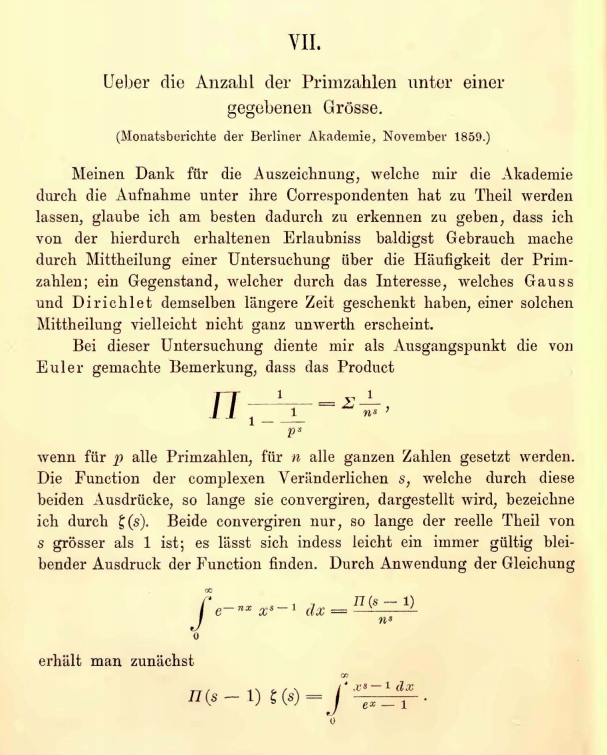
\includegraphics[width=\textwidth]{img/ueber}
\end{column}
\end{columns}
\end{frame}

\begin{frame}{The Riemann zeta function: What Riemann did}
In his paper Riemann takes the function $\zeta\colon \{\sigma + it \in\mathbb{C}\mid \sigma > 1\} \to \mathbb{C}$ and extends it to all of $\mathbb{C}$.
\end{frame}

%plots

\section{Zeta functions for graphs}
\note{now time for something completely different, the links should become clear shortly.}

\begin{frame}{Ramanujan graphs}
\begin{columns}
\begin{column}{.618\textwidth}

Suppose we want to design a communications network (for computers, people, phones, etc.) by linking together $n$ entities with wires, such that each object has only $k$ wires from it.

\pause We shall call our entities \emph{nodes} and wires \emph{edges}, as in graph theory.

\note{There are several properties of such a network we could want}
\pause For today we will think of our goal as the following:

If we split our network into two nonempty parts (a partition) there should be lots of edges between the two halves. \note{so lots of messages can get through simultaneously}
\end{column}
\begin{column}{.3819\textwidth}

\tikzstyle{every node}=[circle, draw, fill=black!50,
                        inner sep=0pt, minimum width=4pt]
\pause
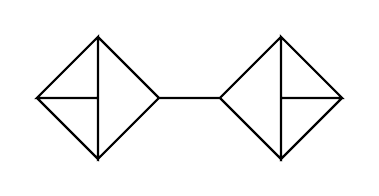
\begin{tikzpicture}[thick,scale=0.775]%
        \draw (0,0) node{} -- (1,1) node{} -- (2,0) node{}
 -- (3,0) node{} -- (4,1) node{} -- (5,0) node{} -- (4,-1) node{}
 -- (4,0) node{} -- (5,0) node{} -- (4,1) node{} -- (4,0) node{}
 -- (4,-1) node{} -- (3,0) node{} -- (2,0) node{} -- (1,-1) node{}
 -- (1,0) node{} -- (1,1) node{} -- (0,0) node{} -- (1,0) node{}
 -- (1,-1) node{} -- (0,0) node{};
\end{tikzpicture}
\pause
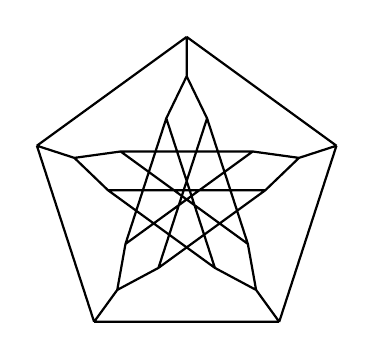
\begin{tikzpicture}[thick,scale=0.5]%
    \draw \foreach \x in {18,90,...,306} {
        (\x:4) node{} -- (\x+72:4)
        (\x:4) -- (\x:3) node{}
        (\x:3) -- (\x+15:2) node{}
        (\x:3) -- (\x-15:2) node{}
        (\x+15:2) -- (\x+144-15:2)
        (\x-15:2) -- (\x+144+15:2)
};
\end{tikzpicture}
\end{column}
\end{columns}
\end{frame}

\begin{frame}{Ramanujan graphs}
\begin{block}{The Cheeger constant}

\end{block}
\end{frame}

% Sarnark wolf prize
\begin{frame}{The Ihara zeta function}
\begin{block}{}
\end{block}
\end{frame}

\section[More zetas]{More assorted zetas}

\begin{frame}{The zeta function of a scheme}
\begin{block}{}
\end{block}
\end{frame}

\section[Number theory again]{Back to number theory}
\begin{frame}{The Dedekind zeta function}
Dedekind wanted to use the 
\begin{block}{}
\end{block}
\end{frame}
\note{didn't want to talk about number theory so much as I wanted to focus more on why you might care about zeta functions even if you don't care about the structure of the primes.}

\section{Conclusion}
\begin{frame}{Closing remarks}
\begin{itemize}
\item Zeta functions can be used to pack up useful information into one big package (a complex function).
\pause\item The properties of this package can be used to discover and prove statements about the objects you started with.
\pause\item We can also see the link different objects via their zeta functions.
\pause\item A huge number of papers have been written that assume the Riemann hypothsis, so a proof of it would imply hundreds of other results true.
\end{itemize}
\end{frame}

\end{document}

% Sources:
% http://graphtheoryinlatex.blogspot.com/
% Sarnark: What is... an expander.

